\documentclass{standalone}

\usepackage{tikz}
\usetikzlibrary{shapes.geometric, arrows,positioning,calc}

\tikzstyle{startstop} = [rectangle, rounded corners, minimum width=2cm, minimum
height=0.5cm, align=center, draw]

\tikzstyle{io} = [trapezium, trapezium left angle=70, trapezium right angle=110, align=center, draw]

\tikzstyle{process} = [rectangle, align=center, draw]

\tikzstyle{oval}=[ellipse, align=center, draw]

\tikzstyle{decision} = [shape aspect=2,diamond, align=center, draw]

\tikzstyle{arrow} = [thick,->,>=stealth]
\tikzstyle{dotArrow} = [dotted, ->, >=stealth]
\tikzstyle{line} = [-]



\usetikzlibrary{decorations.pathreplacing}

\begin{document}
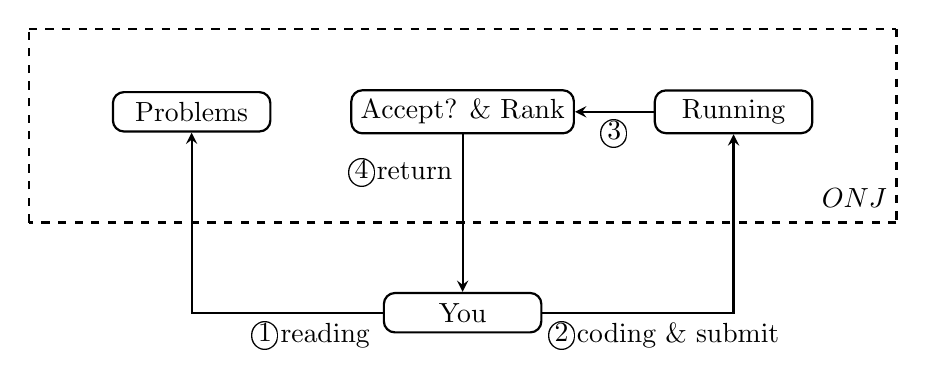
\begin{tikzpicture} [node distance=1cm, thick]
  \node (results) [startstop] {Accept? \& Rank};
  \node (problems) [startstop, left=of results] {Problems};
  \node (running) [startstop, right=of results, label={[anchor=south
    east, inner sep=1.5pt, xshift=1cm, yshift=-1cm]south east:$ONJ$}] {Running};
  \node (you) [startstop, below=of results, yshift=-1cm] {You};

  \draw[arrow] (you) -| node[below, xshift=1.5cm]{\textcircled{1}reading}(problems);
  \draw[arrow] (you) -| node[below, xshift=-.9cm]{\textcircled{2}coding \&
    submit}(running);
  \draw[arrow] (running) -- node[below]{\textcircled{3}}(results);
  \draw[arrow] (results) -- node[left, yshift=.5cm]{\textcircled{4}return} (you);

  \draw[dashed] ($(running.east) + (3em, 3em)$) -- ($(running.east) + (3em,
  -4em)$);
  \draw[dashed] ($(running.east) + (3em, -4em)$) -- ($(problems.west) + (-3em,
  -4em)$);
  \draw[dashed] ($(problems.west) + (-3em, -4em)$) -- ($(problems.west) + (-3em,
  3em)$);
  \draw[dashed] ($(problems.west) + (-3em, 3em)$) -- ($(running.east) + (3em,
  3em)$); 
  
  
\end{tikzpicture}


\end{document}



%%% Local Variables:
%%% mode: latex
%%% TeX-master: t
%%% End:
